\documentclass[aps,pra,twocolumn,amsmath,amssymb,nofootinbib,superscriptaddress]{revtex4}

\newcommand{\bra}[1]{\langle#1|}
\newcommand{\ket}[1]{|#1\rangle}
\newcommand{\op}[2]{\hat{\textbf{#1}}_{#2}}
\newcommand{\dagop}[2]{\hat{\textbf{#1}}_{#2}^\dag}
\usepackage[pdftex]{graphicx}
\usepackage{mathrsfs}
\usepackage[colorlinks]{hyperref}

\begin{document}

\bibliographystyle{apsrev}

%
% Title
%

\title{Efficient verification of boson-sampling with tunable phases and observation of the transition from easy to hard instances}

%
% Authors
%

%\author{Keith R. Motes}
%\affiliation{Centre for Engineered Quantum Systems, Department of Physics and Astronomy, Macquarie University, Sydney NSW 2113, Australia}

\author{Peter P. Rohde}
\email[]{dr.rohde@gmail.com}
\homepage{http://www.peterrohde.org}
\affiliation{Centre for Engineered Quantum Systems, Department of Physics and Astronomy, Macquarie University, Sydney NSW 2113, Australia}

\author{Alberto Peruzzo}
\affiliation{School of Physics, The University of Sydney, Australia}

\date{\today}

\frenchspacing

%
% Abstract
%

\begin{abstract}
\end{abstract}

\maketitle

%
% Body
%

Boson-sampling is only a computationally hard problem for certain classes of linear optics networks. Additionally, verifying boson-sampling is itself a hard problem. That is, if an experimentalist provides experimentally obtained samples, just verifying the correctness of those samples is in general computationally complex. This raises two important questions: (1) are there easy and efficient ways to verify the operation of a boson-sampling device?; and (2) is it possible to observe a transition in the computational complexity of a boson-sampling device as the unitary is adjusted between easy and hard instances? Here we will address these two questions using a tunable boson-sampling architecture. Whilst the architecture requires dynamic control, the requirements are modest. With only a single dynamically controlled phase-shift we are able to tune the device between implementing the trivial identity operation (which can be efficiently verified), and a `maximally mixing' operation, which we argue is likely to be computationally hard.

The architecture we consider comprises a unitary of the form $U = HDH$, where $H$ is the 4-mode Hadamard gate
\begin{equation}
H = \frac{1}{2} \left(\begin{array}{cccc}
1 & 1 & 1 & 1 \\
1 & -1 & 1 & -1 \\
1 & 1 & -1 & -1 \\
1 & -1 & -1 & 1
\end{array}\right),
\end{equation}
and $D$ is a diagonal matrix comprising independent phase-shifts on each mode,
\begin{equation}
D = \left(\begin{array}{cccc}
e^{i\phi_1} & 0 & 0 & 0 \\
0 & e^{i\phi_2} & 0 & 0 \\
0 & 0 & e^{i\phi_3} & 0 \\
0 & 0 & 0 & e^{i\phi_4} \\
\end{array}\right).
\end{equation}
The architecture is shown in Fig.~\ref{fig:HDH_decomposition}.
\begin{figure}[!htb]
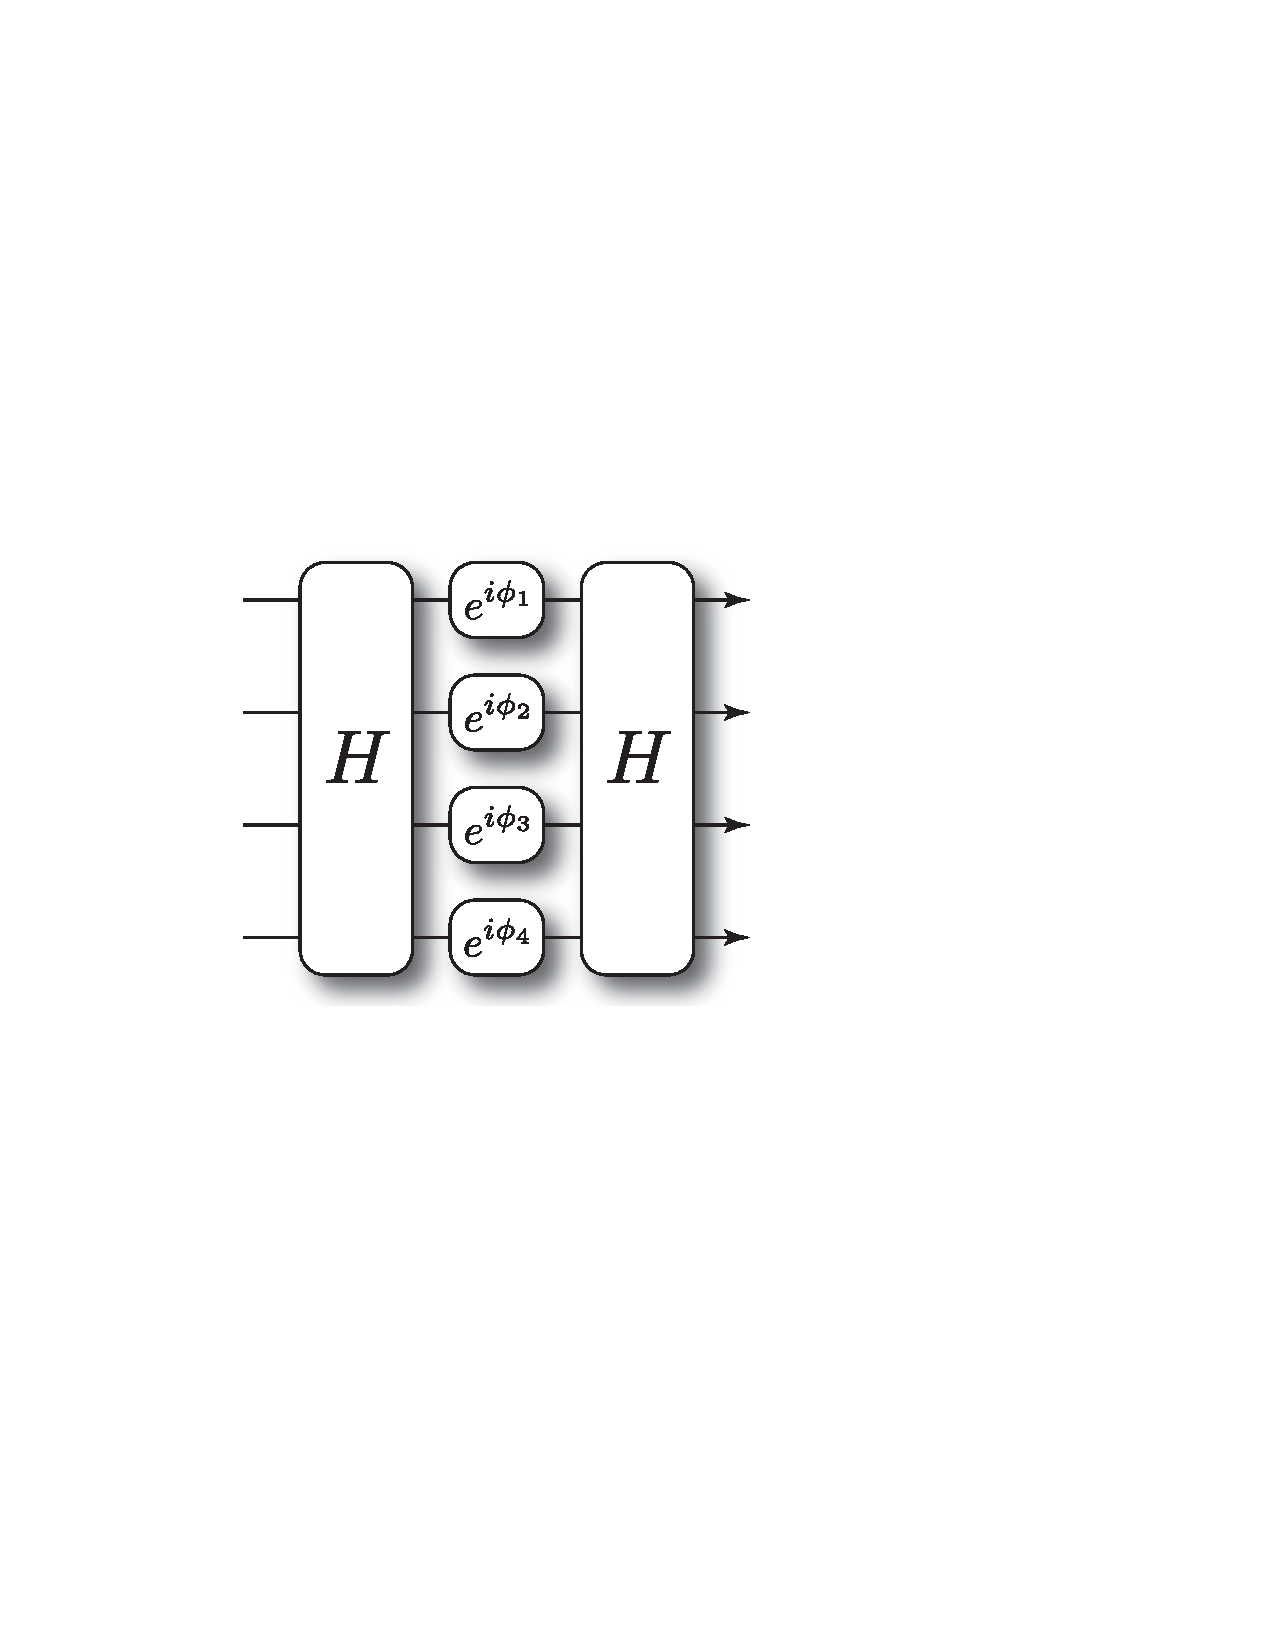
\includegraphics[width=0.5\columnwidth]{HDH_decomposition}
\caption{The $HDH$ architecture, comprising two 4-mode Hadamard operations and four single-mode phases.} \label{fig:HDH_decomposition}
\end{figure}

If we let the phases be $\phi_1=\phi_2=\phi_3=\phi_4=0$, then $U = HIH = I$, and the network implements the trivial identity operation. For non-trivial phases the network is in general highly entangling. To characterize the `hardness' of the network, we employ the `mixing metric' introduced by Motes \emph{et al.}, defined as
\begin{equation}
m(U) = \frac{1}{64} \left(\sum_{i,j=1}^4 |U_{i,j}|\right)^2.
\end{equation}
This metric quantifies how uniform input-to-output amplitudes are for the unitary. When $|U_{i,j}|^2 = 1/4 \,\,\forall\,\, i,j$, the probability amplitude between every input-output pair is balanced, which we call `maximally mixing'. On the other hand, when the unitary is a trivial, non-entangling identity or permutation matrix, the mixing metric is minimized to $1/4$. It was argued by Motes \emph{et al.} that the mixing metric relates to how `hard' a boson-sampling instance is likely to be. When the mixing metric is minmized the combinatorics associated with calculating amplitudes in the output superposition are trivial, whereas for maximally mixing unitaries the combinatorics are maximized.

For our $HDH$ architecture, we find that the mixing metric is of the form,
\begin{eqnarray}
m(HDH) &=& \frac{1}{64} (|e^{\phi_1}+e^{\phi_2}-e^{\phi_3}-e^{\phi_4}| \nonumber\\
&+& |e^{\phi_1}-e^{\phi_2}+e^{\phi_3}-e^{\phi_4}| \nonumber\\
&+& |e^{\phi_1}-e^{\phi_2}-e^{\phi_3}+e^{\phi_4}| \nonumber\\
&+& |e^{\phi_1}+e^{\phi_2}+e^{\phi_3}+e^{\phi_4}|)^2
\end{eqnarray}
When $\phi_1=\phi_2=\phi_3=\phi_4=0$, then $HDH = I$, and $m(I)=1/4$, the minimum value. But when $\phi_1=\phi_2=\phi_3, \phi_4=\pi$,
\begin{equation} \label{eq:max_mix_unitary}
HDH = \frac{1}{2} \left(\begin{array}{cccc}
1 & 1 & 1 & -1 \\
1 & 1 & -1 & 1 \\
1 & -1 & 1 & 1 \\
-1 & 1 & 1 & 1
\end{array}\right),
\end{equation}
$m(U) = 1$, and the mixing metric is maximized. Note that these two instances differ only by the parameter $\phi_4$.

Let us fix $\phi_1=\phi_2=\phi_3=0$, and let $\phi_4$ be variable. Then,
\begin{equation}
m(HDH) = \frac{1}{64}\left(3|1-e^{i\phi_4}| + |3+e^{i\phi_4}| \right)^2.
\end{equation}
Then we have a system in which the entire architecture is fixed, bar a single variable phase, which is dynamically controlled. Control over this phases allows us to tune between the trivial identity operation and the maximally mixing operation from Eq.~\ref{eq:max_mix_unitary}. Thus, by adjusting $\phi_4$, we are able to observe a transition between a trivial and hard instance of boson-sampling. This is illustrated in Fig.~\ref{fig:mixing_fixed_phi4}.
\begin{figure}[!htb]
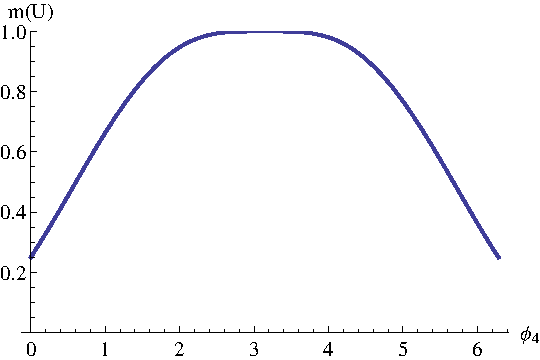
\includegraphics[width=0.8\columnwidth]{mixing_fixed_phi4}
\caption{The mixing metric for $\phi_1=\phi_2=\phi_3=0$ with tunable $\phi_4$, for the $HDH$ architecture.} \label{fig:mixing_fixed_phi4}
\end{figure}

In general, characterizing a boson-sampling device is itself a computationally hard problem as there are an exponential number of terms in the output superposition, the amplitude for each of which must be characterized. Let us set $\phi_4=0$. Then, we have the trivial identity operation and the fidelity of the device is given by the probability that the output state is equal to the input state -- only a single amplitude needs to be characterised. Having performed this verification on the trivial operation, we then tune $\phi_4=\pi$, which yields the maximally mixing unitary. The architecture is fixed and has not changed, bar the change in $\phi_4$, thus we expect the fidelity of the maximally mixing case to be equal to the fidelity of the previously characterized trivial case, allowing us to efficiently characterize the operation of the non-trivial boson-sampling device.

In our $HDH$ architecture, we are able to observe the transition between easy and hard instances of boson-sampling. By characterizing the easy instance, and then tuning the phase to the hard instance, we have effectively characterized the hard instance.

%
% Acknowledgments
%

\begin{acknowledgments}
This research was conducted by the Australian Research Council Centre of Excellence for Engineered Quantum Systems (Project number CE110001013).
\end{acknowledgments}

%
% Bibliography
%

\bibliography{bibliogrpahy}

\end{document}
